The purpose of the study is to quantitatively and qualitatively evaluate
the effectiveness of \tool compared to the DAG-based visualizations
found in Gitk or the git command line. The study is broken into three
task-based sections; conceptual tasks, summarization tasks, and
participant opinions. The study was performed in June of 2017 in
Kingston ON, in a controlled environment running Ubuntu 14.04.
Participants were allowed to use both Gitk and the git command line
tools together, which we will refer to as the git tools. Then they were
asked to perform the same tasks using \tool.

\evan{Do I need to say where the study took place? I see it showing up
  in other papers, but it makes it kind of obvious about the lab I'm
  talking about, doesn't it?}

The primary goal of the study is to determine if \tool is more capable
of providing the participants of our study with a better conceptual
understanding of how a commit is integrated into the kernel, and a
better summarization of various metrics about the files and authors
involved with the integration. The conceptual questions are to determine
if the DAG visualization provides enough information to determine how a
commit, and any related commits, are merged into a project. \tool
displays this information directly in the form of a tree, so we will not
be performing a comparison on this section, only evaluating the results
from Gitk. The summarization tasks compare \tool and Gitk, with the
participants using one tool followed by the other on two commits from
merge-trees of differeing sizes. In both of these sections, the
participant is given a task that they are to find an answer to; we
evaluate the time it took, if the answer was correct, and how far from
the right answer they were. The user opinions provide us with a clear
comparison between the tools from the point-of-view of the participant,
providing us information about which aspects of each tool they prefered.

% TODO: Add the participant profile

\subsection{Tasks}
\label{sub:tasks}

% \dmg{use tasks, not questions. you are asking them to do something that requires an answer, that is different than a question}

\textbf{The conceptual tasks} are designed to gain better insight on the
comprehension of the DAG, and determine if the DAG is sufficient for
understanding what other commits are related to a given commit, and how
those commits are merged. The tasks are outlined in
Table~\ref{tab:conceptual_tasks}. The tasks are performed in order
using the git tools. T1 has the participant draw a diagram of the merge
tree, which will be used to answer the other two questions. This enables
us to visually see issues with comprehending the DAG visualizations.
Participants are given 10 minutes to perform this task, which also is
used to familiarize the participant with the git tools interface, if
they are not already, and with the set of commits they will be working
with. T2 and T3 are drawn directly from the diagram from T1, giving
quantitative metrics to measure the comprehension. T2 asks the
participant to verify the number of commits, and T3 asks for the number
of merges. The three tasks are performed on both commits before
continuing to the summarization tasks.

\begin{table*}[htpb]
  \centering
  \caption{Conceptual Tasks }
  \label{tab:conceptual_tasks}
  \begin{tabulary}{0.9\textwidth}{LL}
    \toprule
    Task & Description\\
    \midrule
    T1 & Draw a diagram showing how this commit was merged into the master branch, along with any other related commits\\
    T2 & How many individual commits are related to this commit?\\
    T3 & How many merges are involved with merging this commit into the master branch?\\
    \bottomrule
  \end{tabulary}
\end{table*}

\textbf{The summarization tasks}, listed in Table~\ref{tab:summarization_tasks},
are designed to compare the ability of the participants to summarize
information about the two commits used in the study when using git tools
verses \tool. The tasks are broken into four sets based on what is being
summarized: merges, authorship, files, and modules. The order that the
participants perform each task is randomized within each task set, and
the order of the task sets are then randomized with the exception of the
merges task set which will always come first. We measure and evaluate
three metrics for each task: correctness, accuracy, and timing.
Correctness measures whether the answer was correct or incorrect.
Accuracy measures how far from being correct the provided answer was.
Timing is the duration, in seconds, that the participant took to answer
the task. We begin timing the task at the end of the question, and stop
timing before the last modification to the answer. For this reason, it
is possible for times to overlap between tasks if the participant
changes their answer after answering another question. This will also
modify the answer used for measuring the accuracy. We measure the timing
from the screen capture.

\evan{Is this better, or do you still want me to move the information
  about the randomization to the bottom?}

\begin{table}[htpb]
  \centering
  \caption{Summarization Tasks}
  \label{tab:summarization_tasks}
  \begin{tabulary}{\linewidth}{LLL}
    \toprule
    Task Set   & Task & Description\\\midrule
    Merge      & T4   & What is the series of merges involved with merging this
    commit?\\
    & T5   & What other commits are merged?\\
    Authorship & T6   & How many authors are involved?\\
    & T7   & Who contributed the most changes?\\
    Files      & T8   & How many files were modified?\\
    & T9   & Which file had the most changes?\\
    Modules    & T10  & Which modules does this merge tree involve?\\
    \bottomrule
  \end{tabulary}
\end{table}


While the merge task set is part of the summarization task group, it
works less with the summarization of the commits and more with
comprehension of the models. The task is designed with two goals in
mind; first we want to measure and define which commits and which merges
the participant has defined to be in the merge tree; second to help
solidify which commits and merges will be used in the merge tree.

T4 provides a concrete series of merges that the participant believes to
be integrating the commit into the repository. T5 provides a concrete
set of commits that are related to the commit. We place these tasks
first as the answers to these will be necessary for the participant to
answer the tasks that follow, specifically finding the merge into the
master branch. T6 and T7 are related to the authorship at merges,
determining how many authors are involved and who made the most changes.
T8 and T9 are related to the files that were modified in the merge,
determining how many files were modified and which file had the most
changes. T10 is related to the modules that were modified in the merge.
Modules are not explicitly defined in git, but are a property of the
Linux repository that we noticed while looking at various commits. To
find the modules, take the text up to the first colon in the git log
preview. For the log preview \textit{``ALSA: kernel docs: fix
  sound/core/ kernel-doc''} the module is \textit{``ALSA''}, e.g.

The accuracy metrics are measured slightly differently between tasks due
to different requirements and structures in the answer. In task T4, both
the order and the merges are important. We define the distance to be the
edit distance with insertion, deletion, and transposition at unit cost.
The accuracy is the minimum edit distance necessary to make the answer
correct. T5, T9, and T10 are concerned with the set of elements in the
response; the order is not important. We use the Levenshtein distance,
with insertion, deletion, and substitution of unit cost, from the
provided answer to the correct answer. The answers to T6 and T8 are
single number values; the distance is measured as the absolute value of
the difference between the provided answer and the correct answer. T7
has only a single correct answer, thus the distance would either be zero
or one. For this reason, it is acceptable to omit the accuracy metric
from this task. The correctness metric is simply whether the answer was
correct or not; an accuracy of zero indicates a correct answer.

\textbf{The user-opinion} questions, listed in
Table~\ref{tab:opinion_questions}, are designed to determine which tool
provides a better user experience for summarization and comprehension
tasks, and what aspects of each assisted with their understanding. T11
asks for the preference of the participant, given that their goal is
comprehension and summarization. % TODO add T11 results
We recognize that neither tool is perfect, and participants may have
complaints about both tools, but are interested in what parts of each
tool assisted them with understanding the events in the repository. T12
is meant to address this. % TODO add T12 results


\begin{table}[htpb]
  \centering
  \caption{User-Opinion Questions}
  \label{tab:opinion_questions}
  \begin{tabulary}{0.9\linewidth}{LL}
    \toprule
    Task & Description\\
    \midrule
    T11 & Given these tasks again, which tool would you prefer?\\
    T12 & Which aspects of each tool did you like and why?\\
    \bottomrule
  \end{tabulary}
\end{table}


\subsection{Commit Selection}
\label{sub:commit_selection}

We include two commits in the study to detect differences between merge
tree sizes. The order that the commits are presented to each participant
is randomized. We analyzed the 15096 merge-trees from April 16th 2005 to
October 14th 2014, which corresponds to the releases Linux 2.6.12-rc3
and Linux 3.17-rc1. 25\% of the trees contain at most a single commit
not including the root, while 50\% of the trees contain at most seven
nodes non-root nodes.
% TODO: get the number for this if there is time
75\% of the trees contain at least 51 nodes, and the largest tree
contains 7217 nodes.

From this information, we selected one tree with a single commit, and
one tree with seven other nodes to represent a small tree and a
medium-sized tree. A majority of the trees are flat, where all nodes
merge directly into the root node. Of the 8031 trees containing at least
seven nodes, only 593 contained at least a single internal merge node.
Trivially, trees with a single node cannot have any internal nodes, and
of the 624 trees with seven nodes, only 135 contained at least one inner
node. To increase the complexity of the medium-sized tree, we randomly
selected one of the 135 trees to represent the medium tree.

From the 2008 trees containing only a single node, we selected one at
random, and trivially selected the only commit in the tree. From the
trees containing seven nodes, we selected one randomly, then randomly
selected one of the commits in the tree. We selected commit
\emph{a3c1239eb59c0a907f8be5587d42e950f44543f8} from the tree containing
a single node, which we will refer to as \comA, and commit
\emph{cdbdd1676a5379f1d5cbd4d476f5e349f445befe} from the tree containing
seven nodes, which we will refer to as \comB. A visual representation
for these trees is shown in Figure~\ref{fig:study_commits}.

\begin{figure}[bpt]
  \centering
  \begin{tabular}{ m{1.5cm} m{3cm} }
    
\includegraphics[height=0.5in]{figures/commits/1-commit.pdf} &
    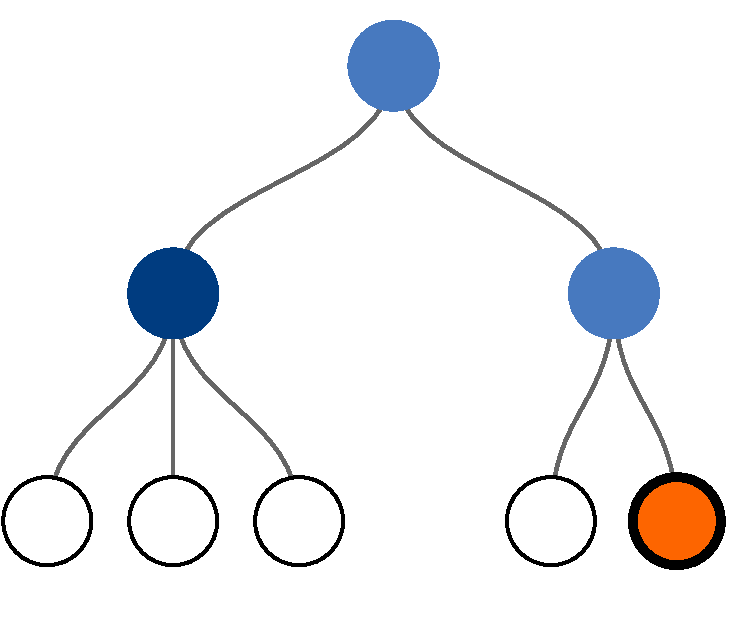
\includegraphics[height=1in]{figures/commits/7-commits.pdf}\\
  \end{tabular}
  \caption{The merge trees used in the user study,
    containing one and seven commits, respectively.}
  \label{fig:study_commits}
\end{figure}

\subsection{Participant Profile}
\label{sub:participant_profile}

The study was conducted with 12 participants, all of whom were
masters, PhD, or post-doc researchers in the field of software
engineering. The participants had between 6 months and 10 years
experience with git, with the median being 3.5 years. Most of the
participants had additional experience with SVN and CVS.\@ One of the
participants in the study worked as a release engineer, studying merge
practices to determine the best way to merge branches while minimizing
the number of merge conflicts, on SVN repositories. The participants
worked with repositories ranging from around 10 commits up to 38000
commits, with the median being 350 commits. Two of the participants had
never collaborated with anyone in a repository, while the rest had some
experience with repositories being modified by multiple people, with the
most being 219. The median number of collaborators was four.

Five participants had only worked with personal and academic
repositories. Two participants had only worked with school and
professional repositories, and two had only worked with professional
repositories. One participant worked with personal, academic, and
professional repositories, one participant had only worked with personal
repositories, and one participant had worked with personal, academic,
and school repositories.

\evan{Do you want more information about the participants?}

All participants have had at least some experience with the idea of
version control, branching in repositories, and git. The participants
are all from the same lab, and each participant worked with both tools
in the study, thus, keeping the sample populations identical for both
tools, with some variation between participants in experience with
repositories.

\subsection{Study Procedure}
\label{sub:study_procedure}

The study begins with a short introduction to the \mt model, followed by
an introduction to Gitk and \tool. We provided two examples of
converting the DAG to the \mt. The first DAG was a flat merge, so the
corresponding merge tree did not have any internal nodes. The second was
not a flat merge, so the corresponding merge tree contained a single
internal node. Any questions about the model were answered at this time.
Following the introduction to the \mt model, we introduce Gitk and
\tool, providing information about what each pane shows in Gitk, and
what each tab does in \tool.

Each task group is applied to both commits, with the order of the commits
randomized between participants to mitigate the effects of order-bias.


The conceptual tasks are the second part of the study. These tasks start
with the participant taking 10 minutes to draw a diagram showing how one
of the commits

% To mitigate the order bias caused by using one tool before the other,
% one commit before the other, and the various tasks, we randomize...

\textbf{Procedure}

\dmg{tell me first why you need to create a script, so I know what you
  do something: we did random assignment of tasks (explain what you did)
  and randomized the order in which the tasks were performed.  Then
  explain why you need a script}

\dmg{it does not randomize the order the tools. It randomizes which tool
  is going to be used on each tasks.  be precise with your language}

\dmg{what you explained how commits relate to tasks and how they get
  assigned? think as if you are explaining this to somebody who has to
  do this: you are the designer, explaining the why and the how }

For each participant, we run a simple python script to generate the
script for the study, eliminating the possibility of bias from us. The
script randomizes the order of the tools, the order of the commits, the
order of the task sets, and the order of the tasks within each task set,
where appropriate.



\subsection{Results}
\label{sec:results}

\dmg{this is still methodology.}
% TODO: Move to methodology
% We recorded the audio and screen capture video for each participant in
% the study for further analysis.
% \dmg{you don't need this sentence, it is redundant}
% After capturing the information, we
% extracted various metrics from the videos.
% \dmg{ you don't record, you measure}
% From the conceptual tasks, we
% recorded the time in seconds, and the answer for the question. We
% extracted three metrics for the summarization tasks, the time in
% seconds, the correctness, and the accuracy.

In task T4, the merges are important, and the order of those
merges is important to the answer. For this task, we use the edit
distance, which will increment if adding merges, removing merges, and
changing the order of the merges is necessary. T5 only asks for the set
of commits, so the order is not important, but the distance will
increase if adding or removing commits is necessary for getting the
correct answer. In T6 and T8 the answer is a single number, so the
distance is simply the difference between the answer provided and the
correct answer. In T7, there is only a single answer that is correct, so
the correctness metric and accuracy are the same, for this reason we do
not measure the accuracy of this task. The answer for T9 is similar in
requirements to T5, only asking for the set of files that had the most
changes. We use the same distance function in T9 and T10 as we did in
T5, measuring the number of items that must be added and removed from
the answer in order to change the response into the correct answer. % TODO: reword
T9 appears to be similar to T7 in that there is only a single file name
that must be provided, but in \comA, two files are modified the same
amount and are both the correct answer. In order to provide the correct
answer, the participant must be able to identify both files. In all
means of accuracy measurement, a correct answer will have a distance of
zero, while a non-zero distance indicates an incorrect answer.


\subsubsection{Conceptual Tasks}
\label{sub:conceptual_tasks}

\dmg{i don't like the expression: we are able to see... too long.. be to the point: Table X shows/depicts/ etc ... they
  are not overviews, they are a summary}
In Table~\ref{tab:conceptual_results}, we are able to see an overview of
the results from the conceptual questions.


\begin{table*}[htpb]
  \centering
  \caption{Results from the conceptual questions\dmg{what are the columns? they need captions}}
  \label{tab:conceptual_results}
  \begin{tabular}{ll|r|lrr|rrr}
    Question                      & Commit & Answer & Median & Mean  & Variance & Median(s) & Mean(s) & Variance(s)\\\hline\hline
    Number of commits in the tree & \comA  & 1      & 4      & 19.11 & 753.11   & 10.0      & 49.92   & 5952.08\\
    Number of merges in the tree  & \comA  & 1      & 5      & 8.27  & 53.62    & 7.5       & 24.67   & 884.42\\\hline
    Number of commits in the tree & \comB  & 5      & 4      & 7.80  & 136.84   & 31.5      & 106.83  & 54123.42\\
    Number of merges in the tree  & \comB  & 3      & 3.5    & 5.40  & 50.27    & 11.0      & 65.6    & 29798.82\\
  \end{tabular}
\end{table*}

Users were able to more closely estimate the number of commits and
merges in the larger tree, but generally took longer than the smaller
tree. The tree with a single node resulted in more variability in the
estimate of number of commits.

It should be noted that these questions were answered after spending
roughly ten minutes attesting to draw a picture that held the answers to
these questions.

\subsubsection{Summarization Tasks}
\label{sub:summarization_tasks}

In Figure~\ref{fig:summarization_results}, we see all of the
correctness, accuracy, and timing results. The first row of plots are
the correctness results. \dmg{be more direct: we see that linvis outperforms gitk by a large margin (then you can
  clarify with the statement you have below; otherwise you are asking the reader to make that connection; don't leave
  that to chance. be explicit on what the results tell you, at the high level.)}
We see in all cases except for T10, that the
number of instances of a correct result with \tool is roughly the same
as the number of incorrect instances with Gitk.
\dmg{you don't test the task. You test what? the statistical significance than one tool is better than the other? Again,
  be explicit}
We test each task with
the McNemar Chi-square test~\cite{McNemar1947}.\dmg{don't break the paragraphs here.. you keep talking about the
  test. If you need to break them, break them before this sentence, not after}

\begin{figure*}[htpb]
  \centering
  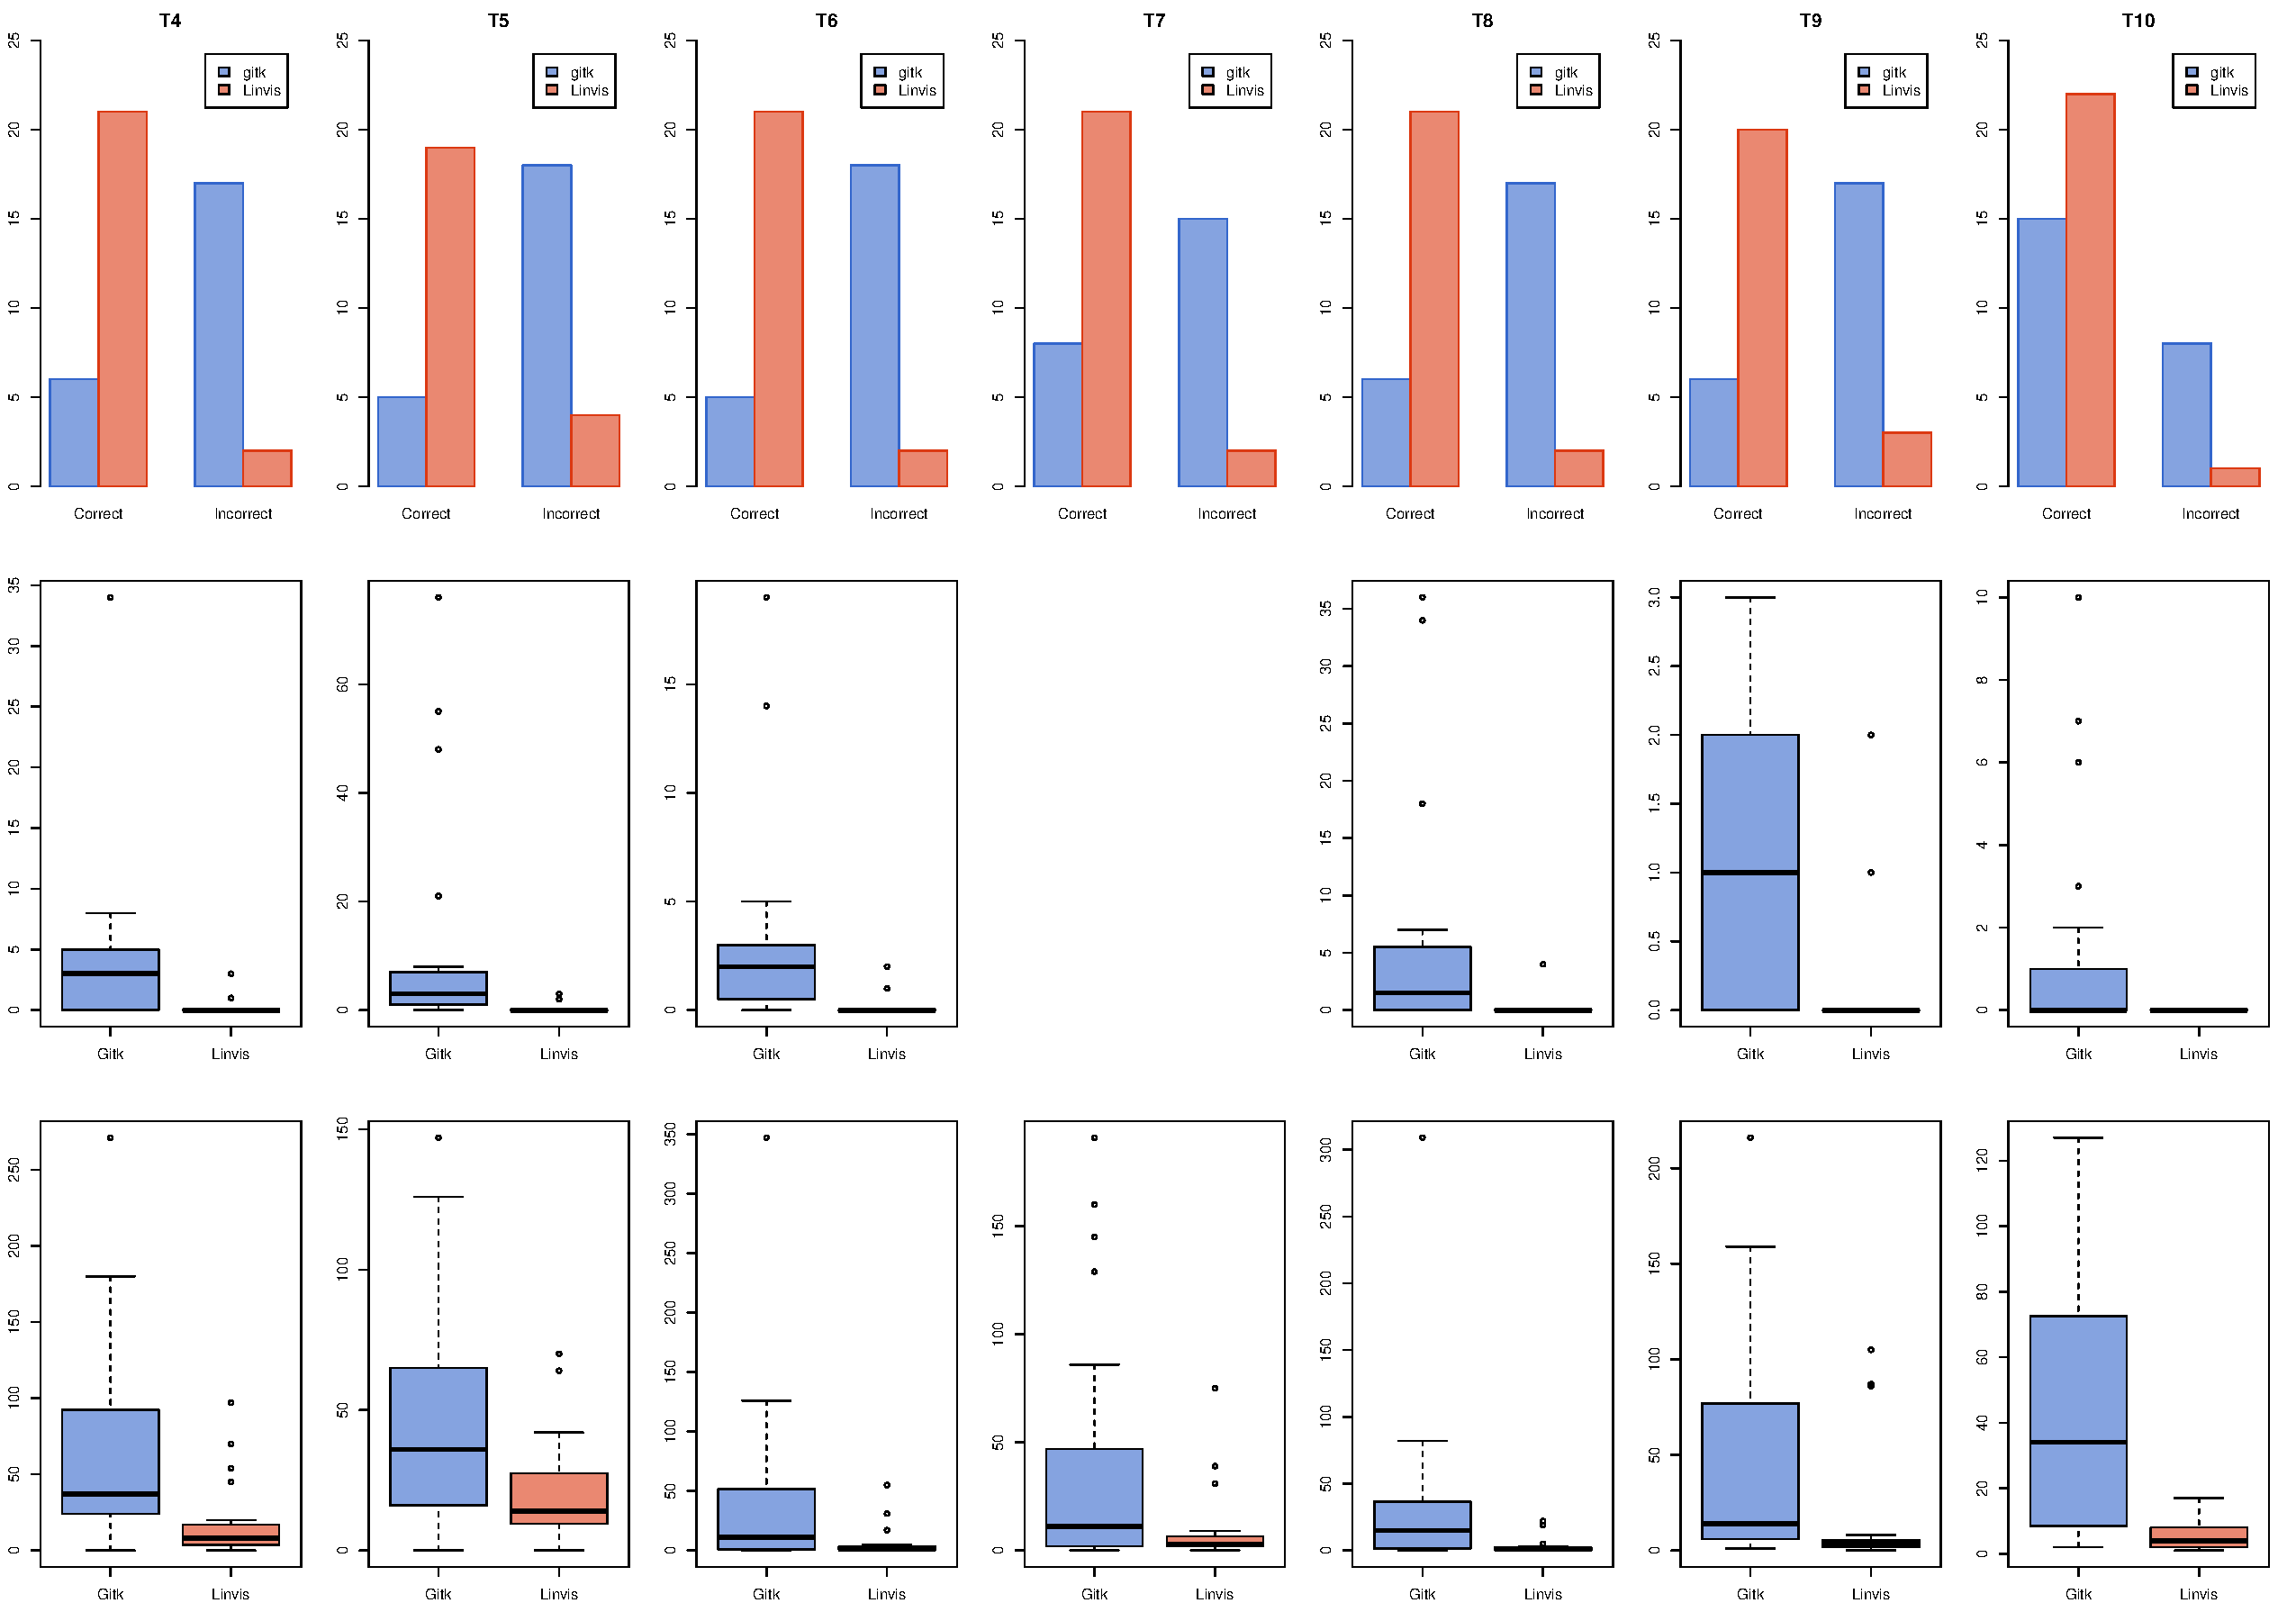
\includegraphics[width=\textwidth]{figures/userstudy/results.pdf}
  \caption{Results from the summarization tasks. The first row plots the
    correctness metric for each task. The second row plots the
    accuracy metric for each task. The third row plots the time metric
    for each task.}
  \label{fig:summarization_results}
\end{figure*}

\dmg{McNemar is used to test if there was an effect on the tool used in the correctness of the answers of the
  users. It is not an analysis of the participants. Don't elaborate on what it does or does not. Just leave it at what
  it does: if you want to be precise you can say it ``marginal homogeneity'' of the answers}

With the McNemar's tests, we analyze the participants that change from
being correct with one tool to being incorrect with the other. \dmg{Again, never, ever, use a pronom like this to start
  a stence. State that this is instead: The McNemar test..., but i vote for removing this info} This does
not take into account the number of people who were able to provide the
correct answer for both tools, nor the people who were incorrect for both
tools. \dmg{this is better, see my comment before this paragraph, you can use this sentence instead, except: not the
  results: the test is used to test the hypothesis that ...} The results show whether providing the participants with \tool
over the current standard, gitk, improves the correctness of the
summarization tasks among the participants. \dmg{Change it to Table shows..., we don't show, we wrote} We show the results for the
number of people who were, with both tools, correct, incorrect, and
changed in Table~\ref{tab:correctness_table}.

In all cases, except for task T10, \dmg{we don't ``see'', ``these is'' instead: in all cases.. there the differences
  are statistically significant} we saw statistically significant
results \dmg{remove suggesting} suggesting that we reject the null hypothesis \dmg{did you tell us what the null hypo
  is?}. \dmg{say this before making conclusions about the results} We tested each
correctness with an $\alpha = 0.005$. The $\chi^2$ test value with one
degree of freedom is $7.879$.\dmg{what is this number? what is it used for? where does it come from?}

\begin{table*}[htpb]
  \centering
  \caption{Correctness tables showing how many people stayed correct,
    incorrect, and how many people changed between tool}
  \label{tab:correctness_table}
  \begin{tabular}{c|c|c}

    T4 & T5 & T6\\
    \begin{tabular}{cc|rr}
      &           & \multicolumn{2}{c}{Linvis}\\
      &           & Correct                      & Incorrect\\\hline
      \multirow{2}{*}{Gitk}  & Correct   & 6                            & 0\\
      & Incorrect & 15                           & 2\\
    \end{tabular} &

    \begin{tabular}{cc|rr}
      &           & \multicolumn{2}{c}{Linvis}\\
      &           & Correct                      & Incorrect\\\hline
      \multirow{2}{*}{Gitk}  & Correct   & 5                            & 0\\
      & Incorrect & 14                           & 4\\
    \end{tabular}

    &

    \begin{tabular}{cc|rr}
      &           & \multicolumn{2}{c}{Linvis}\\
      &           & Correct                      & Incorrect\\\hline
      \multirow{2}{*}{Gitk}  & Correct   & 5                            & 0\\
      & Incorrect & 16                           & 2\\
    \end{tabular}


    \\\hline
    T7 & T8 & T9\\

    \begin{tabular}{cc|rr}
      &           & \multicolumn{2}{c}{Linvis}\\
      &           & Correct                      & Incorrect\\\hline
      \multirow{2}{*}{Gitk}  & Correct   & 8                            & 0\\
      & Incorrect & 13                           & 2\\
    \end{tabular}  &
    \begin{tabular}{cc|rr}
      &           & \multicolumn{2}{c}{Linvis}\\
      &           & Correct                      & Incorrect\\\hline
      \multirow{2}{*}{Gitk}  & Correct   & 6                            & 0\\
      & Incorrect & 15                           & 2\\
    \end{tabular} &
    \begin{tabular}{cc|rr}
      &           & \multicolumn{2}{c}{Linvis}\\
      &           & Correct                      & Incorrect\\\hline
      \multirow{2}{*}{Gitk}  & Correct   & 6                            & 0\\
      & Incorrect & 14                           & 3\\
    \end{tabular}\\\hline

    & T10 & \\
    & \begin{tabular}{cc|rr}
      &           & \multicolumn{2}{c}{Linvis}\\
      &           & Correct                      & Incorrect\\\hline
      \multirow{2}{*}{Gitk}   & Correct   & 14                           & 1\\
      & Incorrect & 8                            & 0\\
    \end{tabular} & \\

  \end{tabular}
\end{table*}

The correctness test statistics and conclusion for each summarization
task;

The correctness test statistics, conclusions, and a description of the
accuracy and timing results for each summarization task follow:

\begin{itemize}

  \item

    T4; the resulting $\chi^2$ value is $15$. $15 > 7.879$, therefore we
    reject the null hypothesis that \tool does not make a difference in
    the correctness when determining the series of merges that a commit
    takes, with $99.5\%$ confidence.

    There is almost no variation in accuracy between participants using
    \tool, while there is more variance in Gitk. There were two outliers
    among the instances using \tool, which lie within the second and
    third quartiles for the accuracy measure of Gitk. The furthest
    outlier for \tool lies at a distance that is slightly greater than
    the median for Gitk.

    We see similar results in the timing metric; all significant data
    occurs within less time than the second, third, and fourth quartile
    of the Gitk results. Nearly all outlier instances in \tool are
    within the third quartile group of the instances of Gitk with the
    exception of the most extreme, which lies in the fourth quartile
    group.

    The results indicate that \tool is able to assist users with
    determining how a commit is merged more accurately, and more
    quickly.

  \item

    T5; the resulting $\chi^2$ value is $14$. $14 > 7.879$, therefore we
    reject the null hypothesis that \tool does not make a difference in
    the correctness when determining the other related commits, with
    $99.5\%$ confidence.

    There is very little variance in the accuracy of results for \tool
    compared to the accuracy of the results in Gitk. The median distance
    is smaller, indicating that the participants performed more
    accurately using \tool.

    There is less variance in the time taken to come to an answer with
    \tool than with Gitk. Furthermore, we see that a majority of the
    participants were able to complete the task in \tool in much less
    time than 50\% of the participants using Gitk.

    The results indicate that \tool is able to assist users in
    understanding which commits are related to a given commit.

  \item

    T6; the resulting $\chi^2$ value is $16$. $16 > 7.879$, therefore we
    reject the null hypothesis that \tool does not make a difference in
    the correctness when determining the number of authors involved with
    the merge tree, with $99.5\%$ confidence.

    We see the same results from this task as with the previous tasks,
    suggesting that \tool assists users determine the number of authors
    more quickly and more accurately.

  \item

    T7; the resulting $\chi^2$ value is $13$. $13 > 7.879$, therefore we
    reject the null hypothesis that \tool does not make a difference in
    the correctness when determining who contributed the most changes,
    with $99.5\%$ confidence.

    This question does not include an accuracy metric, as there are only
    two possible outcomes. We see the same result in the timing metric
    as we did from the previous questions.

    The results suggest that \tool is able to help users correctly
    identify the person who contributed the most lines of code to a
    merge tree in less time.

  \item

    T8; the resulting $\chi^2$ value is $15$. $15 > 7.879$, therefore we
    reject the null hypothesis that \tool does not make a difference in
    the correctness when determining how many files were contributed,
    with $99.5\%$ confidence.

    The results of this task are the same as in the previous tasks.
    This suggest that \tool is able to assist users determine how many
    files were modified, more quickly and more accurately.

  \item

    T9; the resulting $\chi^2$ value is $14$. $14 > 7.879$, therefore we
    reject the null hypothesis that \tool does not make a difference in
    the correctness when determining which file had the most changes,
    with $99.5\%$ confidence.

    While this question appears to have a similar answer to the correct
    answer for T7, the answer \comA had two files with the same number
    of midifications, thus the participant must correctly identify both
    of these files to be correct. For this reason, we include an
    accuracy metric.

    The results of this task are the same as the previous tasks.
    This suggests that \tool is able to assist users to determine which
    file had the most changes.

  \item

    T10; the resulting $\chi^2$ value is $5.44$. $5.44 < 7.879$,
    therefore we do not reject the null hypothesis, suggesting that
    \tool does not make a difference in determining which modules are
    involved with a merge tree.

    The accuracy and timing results for this task are the same as the
    others, showing that there is less variability in both accuracy and
    the time taken to have an answer between participants using \tool
    than using Gitk. Looking Table~\ref{tab:correctness_table}, we can
    see that, unlike the other questions, a majority of the participants
    were correct using both tools.

\end{itemize}

\subsubsection{User Opinions}
\label{sub:user_opinions}

Among the 12 pariticipants, there was nearly unanimous agreement that
for conceptual understanding and summarization tasks, \tool was easier
to work with than Gitk. The participants cited the ability to abstract
information about the merge from the clean summarization tables and
simple visualizations. Three participants suggested that someone with a
professional understanding of Gitk and the git commandline may be to
extract the a good conceptual understanding from the DAG, and perform
the summarization tasks from the commandline. One of these three
participants said that they would prefer to have both tools available,
as they are able to complement each other.

